\documentclass[11pt, a4paper, fontset=none]{ctexart}

\usepackage{experiment_style}

\begin{document}

% =========================================
% P290. Q1
% =========================================
\begin{problem}{P290. Q1}
    先作图分析方程
    \[
        x^2+\sin(10x)-1=0
    \]
    的有根区间，再用弦截法求其在 $[-2,2]$ 内的全部实根。
\end{problem}

\begin{solution}
    \textbf{实验内容、步骤及结果}

    统一根求解函数 \texttt{chap-8/iterative\_root\_finding.m}：

\begin{lstlisting}[language=Matlab]
function [result, n, error_est] = iterative_root_finding(phi, x0, tolerance, method, varargin)
    max_iterations = 1000;
    n = 0;

    switch lower(method)
        case 'simple'
            acceleration = varargin{1};
            x = x0;

            while true
                n = n + 1;
                x_old = x;

                switch lower(acceleration)
                    case 'none'
                        x = phi(x);
                    case 'steffensen'
                        x1 = phi(x);
                        x2 = phi(x1);
                        x = x - (x1 - x) ^ 2 / (x2 - 2 * x1 + x);
                    case 'lambda'
                        lambda = varargin{2};
                        x = lambda * phi(x) + (1 - lambda) * x;
                    otherwise
                        error('Invalid acceleration method.');
                end

                error_est = abs(x - x_old);
                if error_est < tolerance || n >= max_iterations
                    break;
                end
            end

        case 'newton'
            f = varargin{1};
            df = varargin{2};
            x = x0;

            while true
                n = n + 1;
                x_old = x;
                x = x - f(x) / df(x);
                error_est = abs(x - x_old);

                if error_est < tolerance || n >= max_iterations
                    break;
                end
            end

        case 'secant'
            f = varargin{1};
            x_prev = x0(1);
            x = x0(2);

            while true
                n = n + 1;
                x_next = x - f(x) * (x - x_prev) / (f(x) - f(x_prev));
                error_est = abs(x_next - x);
                x_prev = x;
                x = x_next;

                if error_est < tolerance || n >= max_iterations
                    break;
                end
            end

        otherwise
            error('Invalid method specified.');
    end

    if n >= max_iterations
        error('Method did not converge within maximum iterations.');
    end

    result = x;
end
\end{lstlisting}

    主程序 \texttt{chap-8/P290\_Q1.m}：

\begin{lstlisting}[language=Matlab]
f = @(x) x .^ 2 + sin(10 * x) - 1;
x = linspace(-2, 2, 10000);
y = f(x);

figure;
plot(x, y);
xlabel('x');
ylabel('f(x)');
title('Plot of f(x) = x^2 + sin(10x) - 1');
grid on;
ylim([-1 1]);
hold on;

r_num = 1;

for i = 1:length(x) - 1
    a = x(i);
    b = x(i + 1);

    if f(a) * f(b) < 0
        [root, ~, ~] = iterative_root_finding([], [a, b], 1e-6, 'secant', f);
        plot(root, f(root), 'ro');
        fprintf('Approximated root No.%d: %f\n', r_num, root);
        r_num = r_num + 1;
    elseif f(a) == 0
        plot(a, f(a), 'bo');
    end
end

hold off;
\end{lstlisting}

    输出结果如下：

\begin{lstlisting}
>> P290_Q1
Approximated root No.1: -1.414209
Approximated root No.2: -1.356265
Approximated root No.3: -0.951883
Approximated root No.4: -0.551333
Approximated root No.5: -0.412101
Approximated root No.6: 0.137591
Approximated root No.7: 0.183038
Approximated root No.8: 0.684372
Approximated root No.9: 0.928678
Approximated root No.10: 1.208723
\end{lstlisting}

    作图结果如下：

    \begin{figure}[htbp]
        \centering
        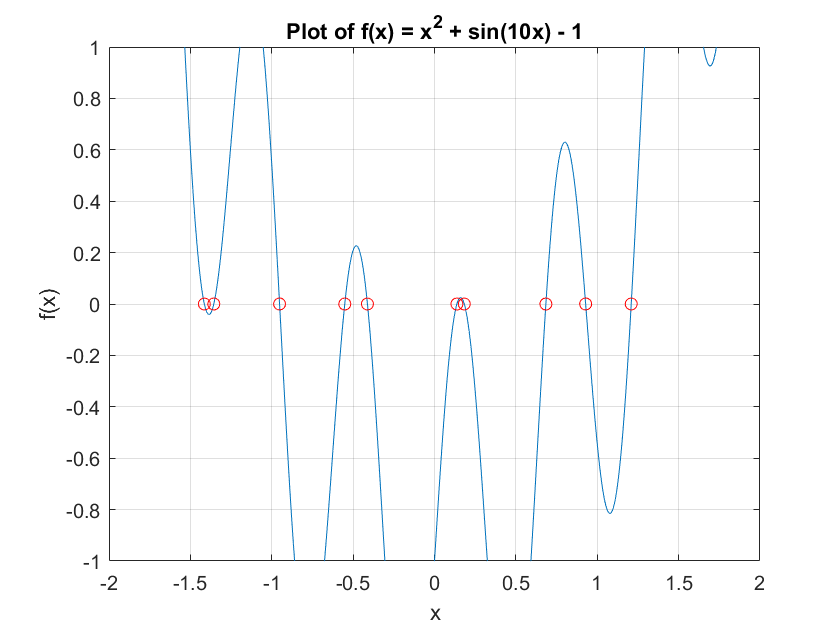
\includegraphics[width=0.82\textwidth]{../../bit-numerical-analysis-hw/chap-8/assets/P290_Q1.png}
    \end{figure}

    \textbf{实验结果分析}

    先在 $[-2,2]$ 上对函数进行密集采样，利用相邻采样点函数值异号判断有根区间，再以该小区间作为割线法初值。计算结果显示方程在 $[-2,2]$ 内共有 $10$ 个实根，图中的红色圆点即为求出的零点。
\end{solution}


% =========================================
% P290. Q2
% =========================================
\begin{problem}{P290. Q2}
    用简单迭代法求方程
    \[
        x=e^{-x}
    \]
    的根，并比较普通迭代与加速迭代的收敛速度。
\end{problem}

\begin{solution}
    \textbf{实验内容、步骤及结果}

    主程序 \texttt{chap-8/P290\_Q2.m}：

\begin{lstlisting}[language=Matlab]
phi = @(x) exp(-x);
[result, n, error_est] = iterative_root_finding(phi, .5, 1e-8, 'simple', 'none');

fprintf('Simple iteration with no acceleration:\n');
fprintf('Approximated root: %f\n', result);
fprintf('Number of iterations: %d\n', n);
fprintf('Error estimate: %e\n\n', error_est);

f = @(x) x - exp(-x);
root_fzero = fzero(f, [0, 1]);
fprintf('Root using fzero: %f\n', root_fzero);
fprintf('Difference between methods: %e\n', abs(result - root_fzero));

[result, n, error_est] = iterative_root_finding(phi, .5, 1e-8, 'simple', 'lambda', 0.625);

fprintf('\nSimple iteration with lambda acceleration:\n');
fprintf('Approximated root: %f\n', result);
fprintf('Number of iterations: %d\n', n);
fprintf('Error estimate: %e\n\n', error_est);

fprintf('Root using fzero: %f\n', root_fzero);
fprintf('Difference between methods: %e\n', abs(result - root_fzero));
\end{lstlisting}

    输出结果如下：

\begin{lstlisting}
>> P290_Q2
Simple iteration with no acceleration:
Approximated root: 0.567143
Number of iterations: 30
Error estimate: 7.733198e-09

Root using fzero: 0.567143
Difference between methods: 2.798615e-09

Simple iteration with lambda acceleration:
Approximated root: 0.567143
Number of iterations: 5
Error estimate: 4.740185e-09

Root using fzero: 0.567143
Difference between methods: 9.938261e-11
\end{lstlisting}

    \textbf{实验结果分析}

    不加速时，迭代函数为
    \[
        \varphi(x)=e^{-x}.
    \]
    从 $x_0=0.5$ 出发需要 $30$ 次迭代达到 $10^{-8}$ 的停止精度。采用松弛形式
    \[
        x_{n+1}=\lambda e^{-x_n}+(1-\lambda)x_n,\qquad \lambda=0.625,
    \]
    只需 $5$ 次迭代即可达到同等精度，说明合适的加速参数能显著改善简单迭代的收敛速度。
\end{solution}


% =========================================
% P290. Q3
% =========================================
\begin{problem}{P290. Q3}
    先作图分析下列方程的有根区间，编写 Newton 法和弦截法程序求解：
    \[
        \text{(1)}\quad 5x^{23}-6x^7+8x^6-5x^2=0,
    \]
    \[
        \text{(2)}\quad e^{-2x+6}\cos(10x)+e^{-3x}\sin(2x)-e^6=0.
    \]
\end{problem}

\begin{solution}
    \textbf{实验内容、步骤及结果}

    第 (1) 题主程序 \texttt{chap-8/P290\_Q3\_1.m}：

\begin{lstlisting}[language=Matlab]
f = @(x) 5 * x .^ 23 - 6 * x .^ 7 + 8 * x .^ 6 - 5 * x .^ 2;
x = linspace(-1, 1, 10000);
y = f(x);

figure;
plot(x, y);
xlabel('x');
ylabel('f(x)');
title('Plot of f(x) = 5x^{23} - 6x^{7} + 8x^{6} - 5x^{2}');
grid on;
hold on;

r_num = 1;

for i = 1:length(x) - 1
    a = x(i);
    b = x(i + 1);

    if f(a) * f(b) < 0
        [root, ~, ~] = iterative_root_finding([], [a, b], 1e-6, 'secant', f);
        plot(root, f(root), 'ro');
        fprintf('Approximated root No.%d: %f\n', r_num, root);
        r_num = r_num + 1;
    elseif f(a) == 0
        plot(a, f(a), 'bo');
    end
end

[root, ~, ~] = iterative_root_finding([], [-1e-1, 1/2], 1e-6, 'secant', f);
plot(root, f(root), 'ko', 'MarkerFaceColor', 'k');
fprintf('Approximated root No.%d: %f\n', r_num, root);

hold off;
\end{lstlisting}

    第 (1) 题输出如下：

\begin{lstlisting}
>> P290_Q3_1
Approximated root No.1: -0.792745
Approximated root No.2: 0.976776
Approximated root No.3: -0.000002
\end{lstlisting}

    作图结果如下：

    \begin{figure}[htbp]
        \centering
        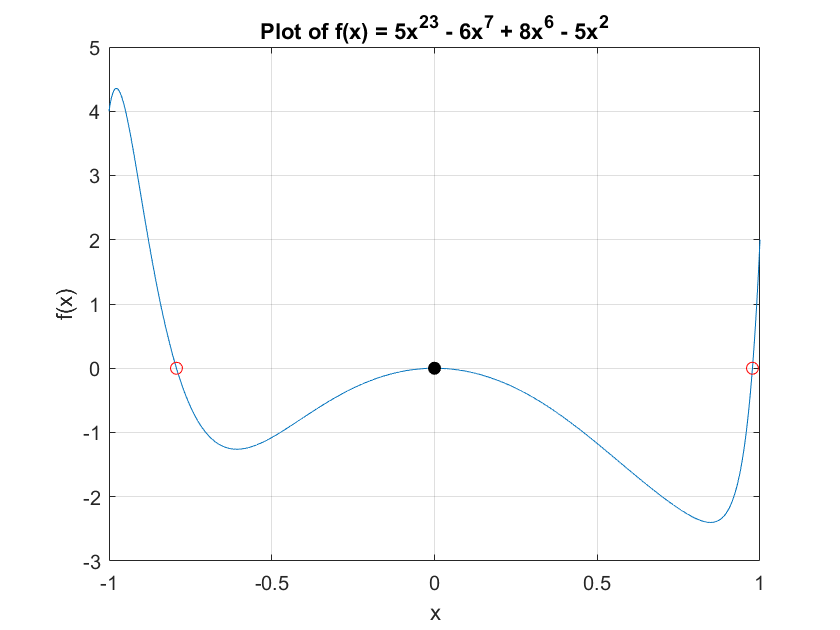
\includegraphics[width=0.82\textwidth]{../../bit-numerical-analysis-hw/chap-8/assets/P290_Q3_1.png}
    \end{figure}

    第 (2) 题主程序 \texttt{chap-8/P290\_Q3\_2.m}：

\begin{lstlisting}[language=Matlab]
f = @(x) exp(-2 * x + 6) .* cos(10 * x) + exp(-3 * x) .* sin(2 * x) - exp(6);
x = linspace(-1, 1, 10000);
y = f(x);

figure;
plot(x, y);
xlabel('x');
ylabel('f(x)');
title('Plot of f(x) = exp(-2x + 6)cos(10x) + exp(-3x)sin(2x) - exp(6)');
grid on;
hold on;

r_num = 1;

for i = 1:length(x) - 1
    a = x(i);
    b = x(i + 1);

    if f(a) * f(b) < 0
        [root, ~, ~] = iterative_root_finding([], [a, b], 1e-6, 'secant', f);
        plot(root, f(root), 'ro');
        fprintf('Approximated root No.%d: %f\n', r_num, root);
        r_num = r_num + 1;
    elseif f(a) == 0
        plot(a, f(a), 'bo');
    end
end

hold off;
\end{lstlisting}

    第 (2) 题输出如下：

\begin{lstlisting}
>> P290_Q3_2
Approximated root No.1: -0.762936
Approximated root No.2: -0.508613
Approximated root No.3: -0.038869
Approximated root No.4: -0.000000
\end{lstlisting}

    作图结果如下：

    \begin{figure}[htbp]
        \centering
        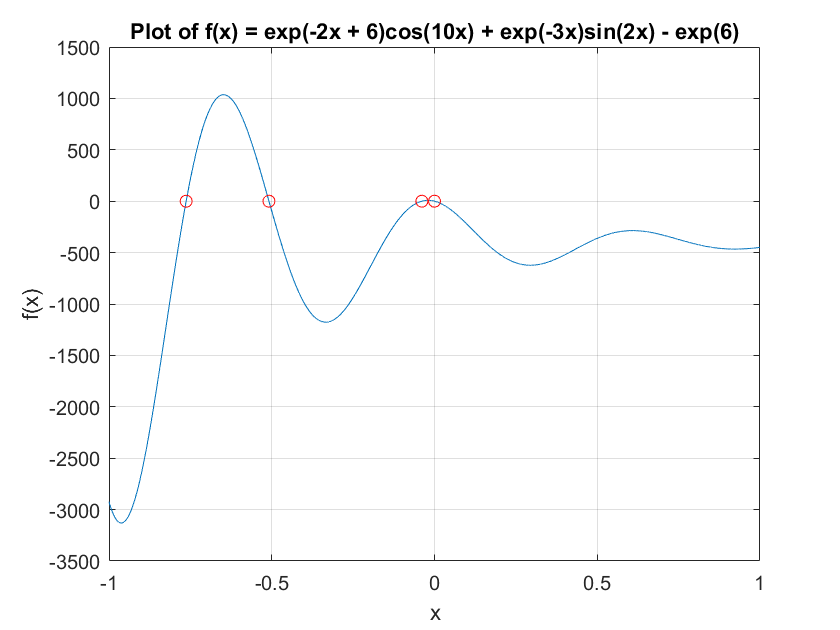
\includegraphics[width=0.82\textwidth]{../../bit-numerical-analysis-hw/chap-8/assets/P290_Q3_2.png}
    \end{figure}

    \textbf{实验结果分析}

    对第 (1) 个方程，作图和采样变号区间能找到两个明显的变号根；由于 $x=0$ 也是根，但在数值采样中不一定出现变号，因此额外选取靠近 $0$ 的启动点用割线法求得该根。对第 (2) 个方程，在 $[-1,1]$ 上可找到 $4$ 个实根，其中 $x=0$ 附近的根也能由割线法稳定逼近。
\end{solution}

\end{document}
